% Appendix Template
\chapter{Appendix} % Main appendix title
\label{appA} % Change X to a consecutive letter; for referencing this appendix elsewhere, use \ref{AppendixX}

\begin{figure}[tbh!]
\centering
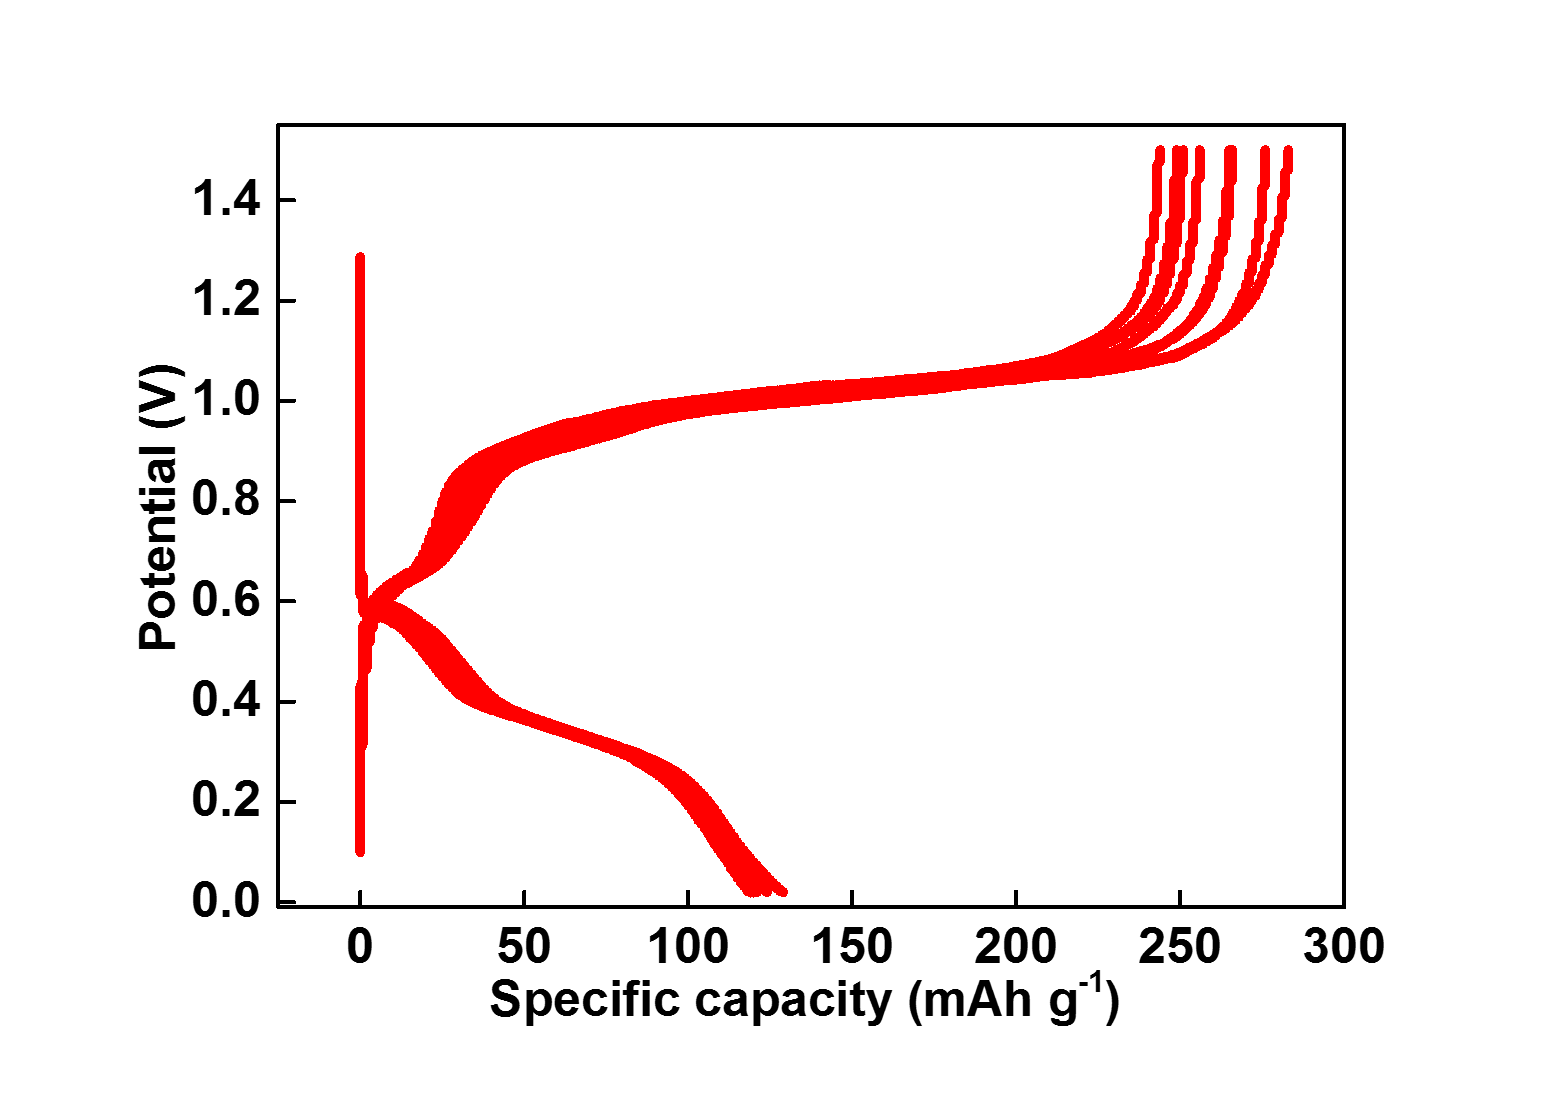
\includegraphics[width=\textwidth]{Figures/appendix/hBNrepeat}
\caption{Galvanostatic charge/discharge curves of an Al/hBN cells using old hBN using a two-electrode setup at a current rate of 40 mA g$^{-1}$. }
\label{Figures/appendix:hBNrepeat}
\end{figure}

\begin{figure}[tbh!]
\centering

\includegraphics[width=\textwidth]{Figures/appendix/pouchCE}
\caption{a) Coulombic efficiency recorded for 1600 cycles of an Al/hBN pouch cell assembled in IKTS, Germany.}
\label{Figures/appendix:pouchCE}
\end{figure}

\begin{figure}[tbh!]
\centering
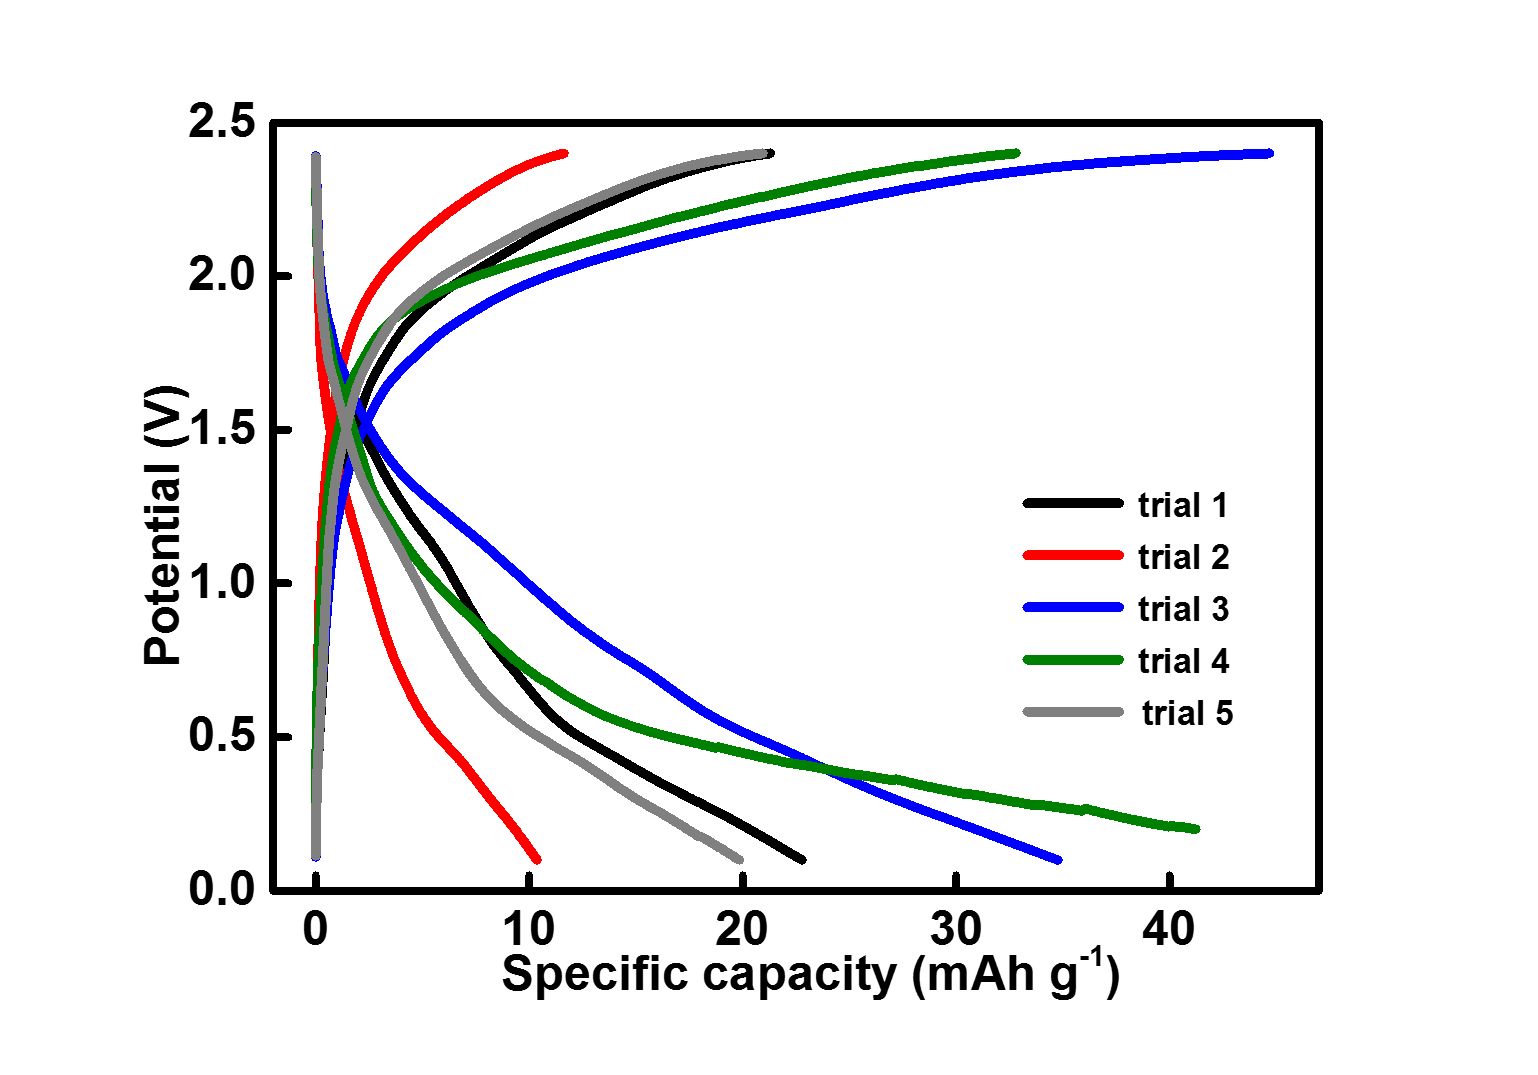
\includegraphics[width=\textwidth]{Figures/appendix/hBNmultiattempts}
\caption{CDCs of Al/hBN cells using pure hBN, 98\% pure, $\approx$1 $\mu$m in size using similar assembly conditions. All cells were run at a current rate of 40 mA g$^{-1}$. Despite repeated attempts, none of the cells recorded a capacity above 50 mAh g$^{-1}$. This was an issue because we were trying to replicate our previous results where an Al/hBN cells recorded capacities above 100 mAh g$^{-1}$, Figure \ref{Figures/appendix:hBNrepeat}.}
\label{Figures/appendix:hBNmultiattempts}
\end{figure}

\begin{figure}[tbh!]
\centering
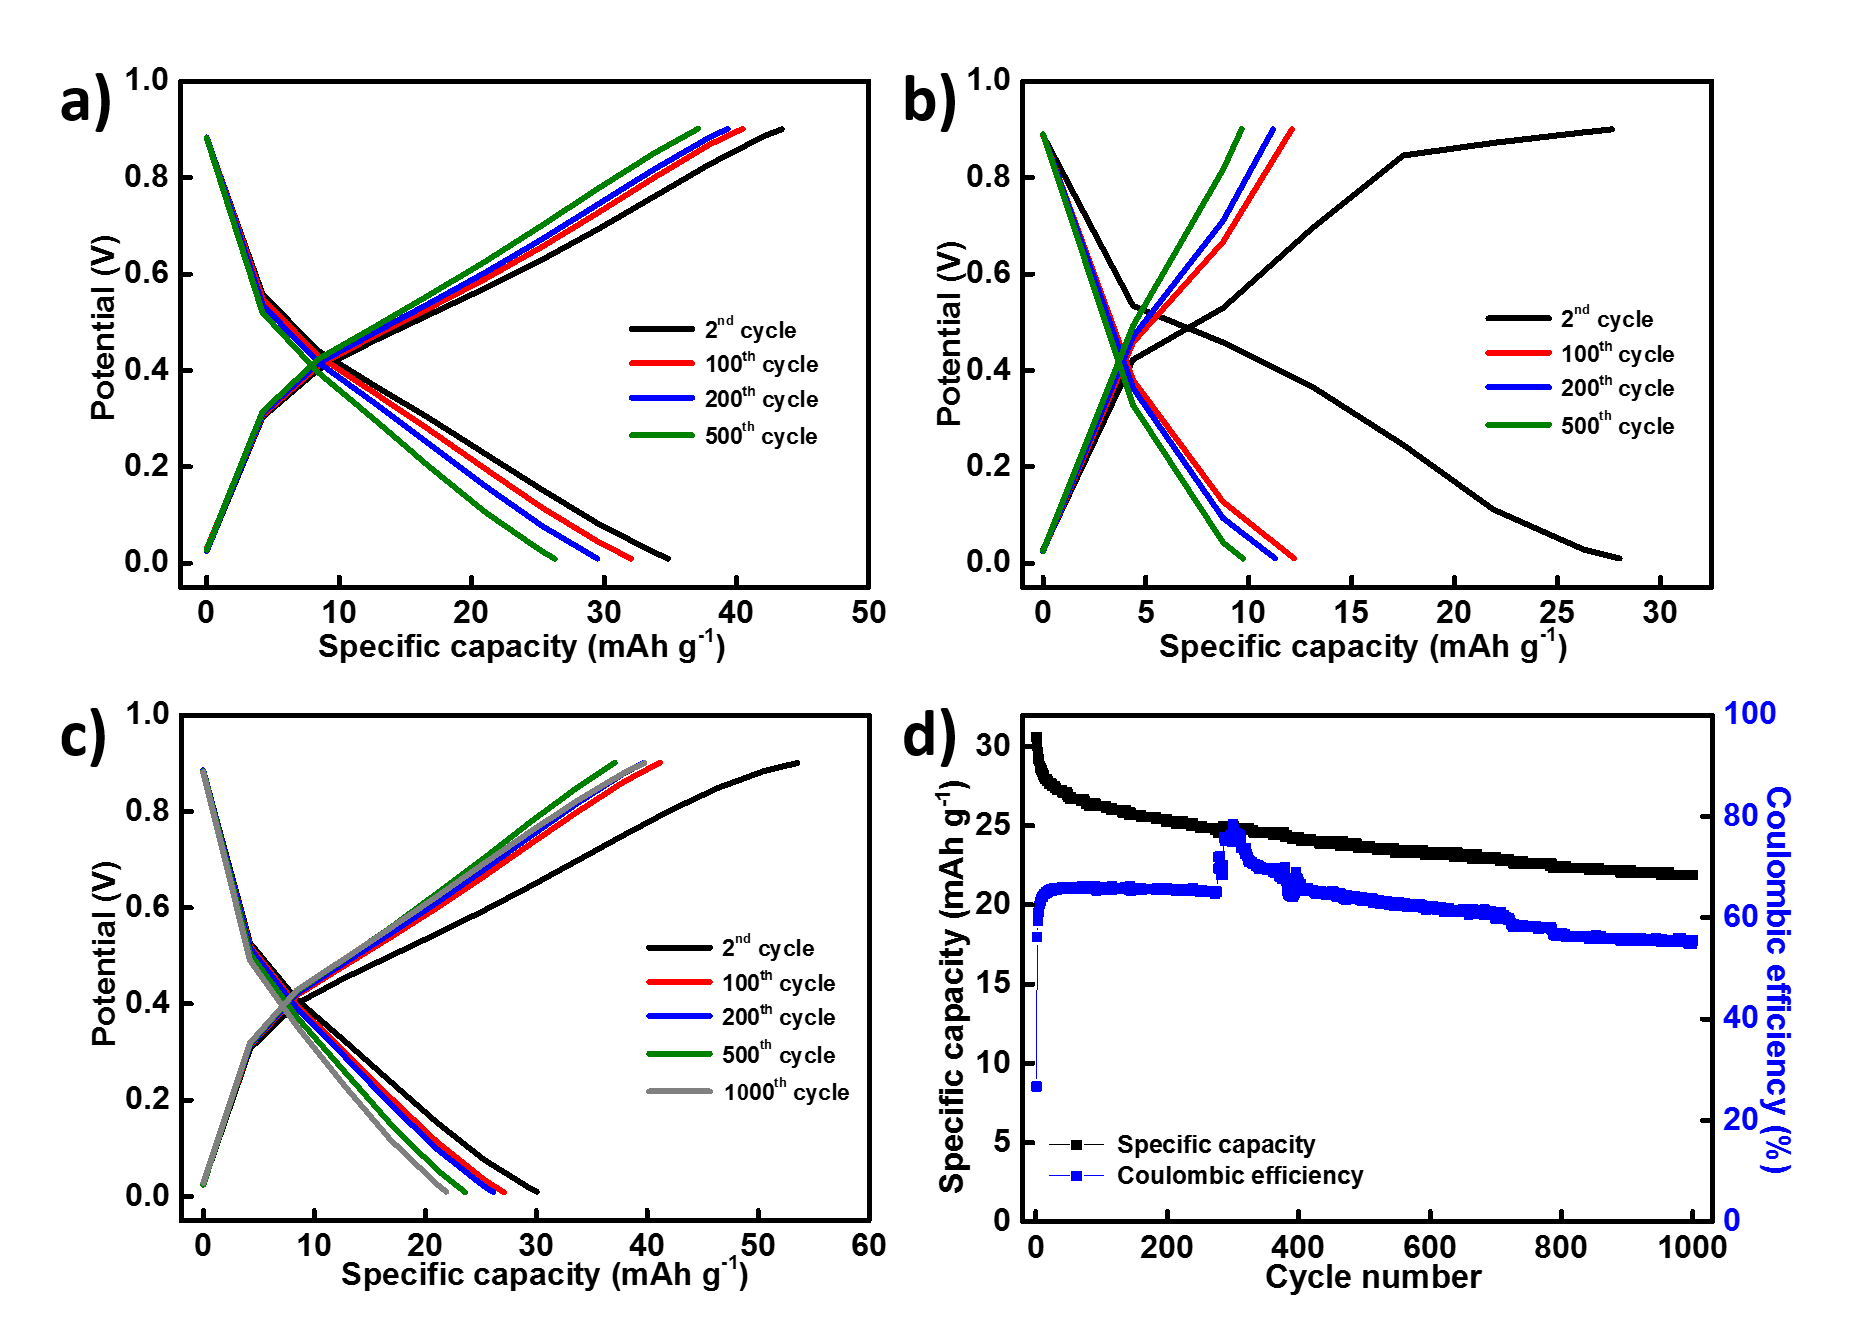
\includegraphics[width=\textwidth]{Figures/appendix/pouchcellCDCCE}
\caption{a-c) Cell performance of various Al/hBN pouch cells assembled in ITKS, Germany. None of the cells managed to achieve capacities above 50 mAh g$^{-1}$. d) Coulombic efficiency of an Al/hBN cell run for thousand cycles at a current rate of 40 mA g$^{-1}$. }
\label{Figures/appendix:pouchcellCDCCE}
\end{figure}
\begin{figure}[tbh!]
\centering
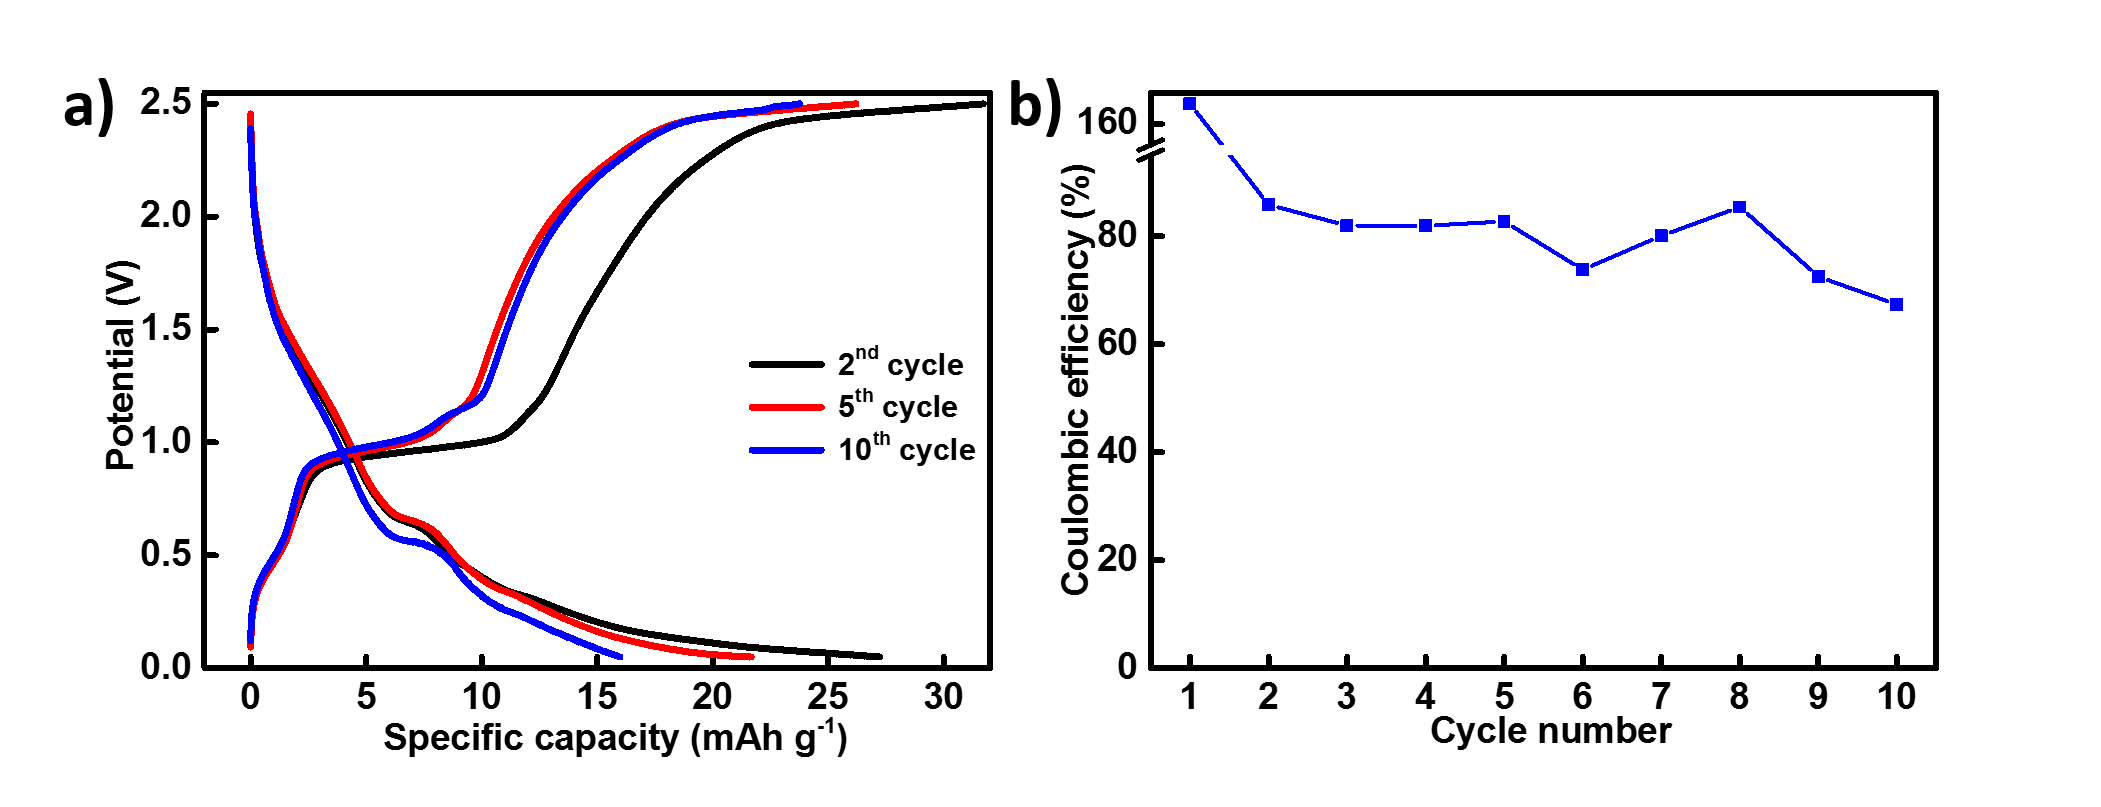
\includegraphics[width=\textwidth]{Figures/appendix/WS2CDCCE}
\caption{ a) Galvanostatic charge/discharge cycles, and b) coulombic efficiency of an Al/\ce{WS2} cell for 10 cycles at a current rate of 50 mA g$^{-1}$. A distinct plateau was seen during discharge at 0.68 V and a charging plateau was observed at 1.0 V vs \ce{Al$^{3+}$}/Al. \ce{WS2} has a layered structure similar to \ce{MoS2} with an interlayer distance of 6.18 \AA. Looking at the CDCs, a few \ce{AlCl4-} ions manage to intercalate but it seems the side reactions taking place at the electrode/electrolyte interface prevent the cell from achieving high specific capacities.}
\label{Figures/appendix:WS2CDCCE}
\end{figure}